%%==========================================================================%%
%% Author : Abascal Fern�ndez, Patricia                                     %%
%% Author : S�nchez Barreiro, Pablo                                         %%
%% Version: 1.1, 21/04/2013                                                 %%
%%                                                                          %%
%% Memoria del Proyecto Fin de Carrera                                      %%
%% Domain Engineering/Ejemplo de Generaci�n de C�digo C#: Caso Complejo     %%
%%==========================================================================%%
Antes de comenzar a exponer los ejemplos m�s complejo, vamos a introducir aquellos conceptos que pasamos por algo en la secci�n \ref{domain:sec:transf} dada su complejidad: las relaciones bidireccionales y la herencia m�ltiple.

 \paragraph{Relaciones Bidireccionales} \ \\
 \begin{figure}[!tb]
  \centering
  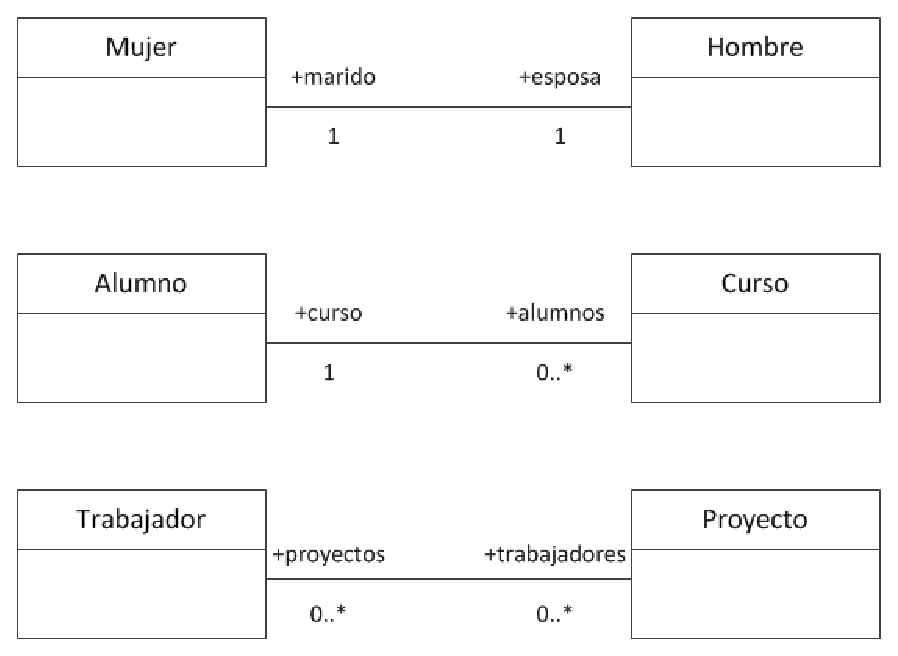
\includegraphics[width=.75\linewidth]{domainEngineering/images/bidireccionales.eps} \\
  \caption{Tipos de relaciones bidireccionales}
  \label{dom:fig:bid}
\end{figure}

Las relaciones bidireccionales son aquellas en las que ambas clases relacionadas disponen de atributos de la clase opuesta. Existen tres tipos de relaciones bidireccionales:
 \begin{itemize}
   \item Bidireccionales one to one, en las que cada clase recibe un elemento de la clase opuesta (figura \ref{dom:fig:bid}, Mujer-Marido).
   \item Bidireccionales one to many, en la que una de las clases recibe un elemento de la clase destino y la otra recibe una colecci�n de elementos de la clase opuesta (figura \ref{dom:fig:bid}, Alumno-Curso).
   \item Bidireccionales many to many, en la que ambas clases reciben colecciones de la clase opuesta (figura \ref{dom:fig:bid}, Trabajadores-Proyectos).
 \end{itemize}

\paragraph{Herencia m�ltiple} \ \\

\begin{figure}[!tb]
  \centering
  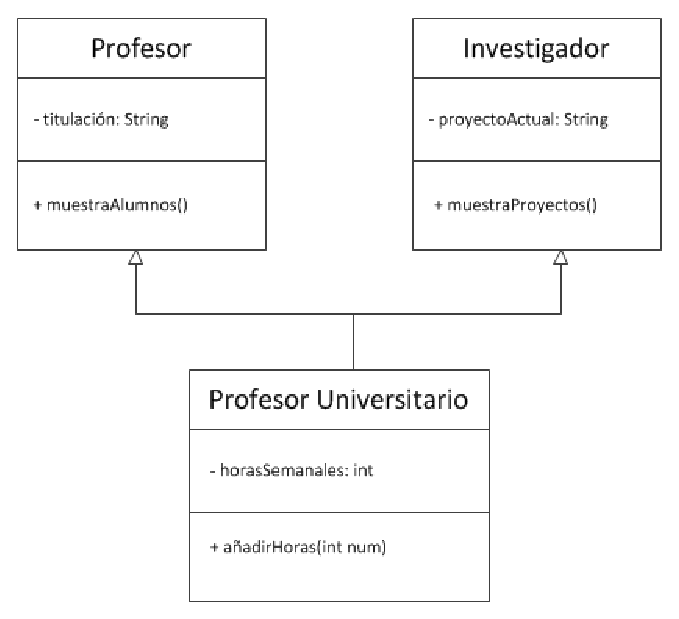
\includegraphics[width=.50\linewidth]{domainEngineering/images/herenciamultiple.eps} \\
  \caption{Tipos de relaciones bidireccionales}
  \label{dom:fig:her}
\end{figure}

 \begin{figure}[!tb]
  \centering
  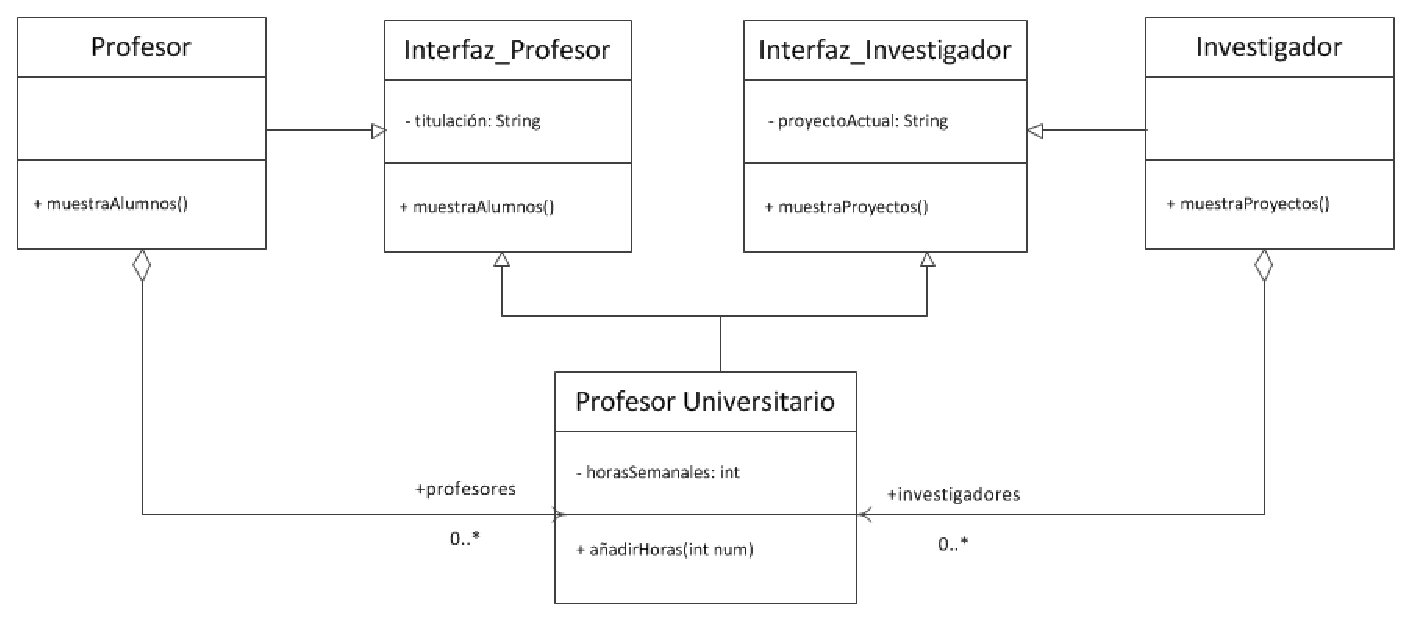
\includegraphics[width=.80\linewidth]{domainEngineering/images/herenciamultiple_implementada.eps} \\
  \caption{Tipos de relaciones bidireccionales}
  \label{dom:fig:hersol}
\end{figure}
Los modelos UML admiten la herencia m�ltiple de clases, pero lenguajes como C\# no por lo que hay que transformar el modelo iniciar para adaptarlo y que funcione correctamente. Podemos encontrarnos con un conjunto de clases como el descrito en la figura \ref{dom:fig:her} donde se puede apreciar que la clase \imp{Profesor Universitario} presenta herencia m�ltiple de las clases \imp{Profesor} e \imp{Investigador}, por tanto debemos procesar la informaci�n de forma que funcione correctamente en C\#, las modificaciones que debemos realizar son:

\begin{itemize}
  \item Por cada una de las clases padre, \imp{Profesor} e \imp{Investigador}, se generan sendas interfaces \imp{Interfaz\_Profesor} e \imp{Interfaz\_Investigador}.
  \item Las clases padre solo contienen los m�todos de la clase y heredan de sus respectivas interfaces.
  \item Las interfaces correspondientes a las clases padre tienen los m�todos y las propiedades de la respectiva clase.
  \item La clase hija, \imp{Profesor Universitario}, hereda ahora de las interfaces \imp{Interfaz\_Profesor} e \imp{Interfaz\_Investigador} en lugar de heredar de las clases \imp{Profesor} e \imp{Investigador} como ocurr�a en el modelo inicial.
  \item La clase hija incorpora, adem�s de sus propiedades y m�todos, colecciones para acceder a las clases \imp{Profesor} e \imp{Investigador}.
\end{itemize}
 